
%%%%%%%% ICML 2018 EXAMPLE LATEX SUBMISSION FILE %%%%%%%%%%%%%%%%%

\documentclass{article}

% Recommended, but optional, packages for figures and better typesetting:
\usepackage{microtype}
\usepackage{graphicx}
\usepackage{subfigure}
\usepackage{booktabs} % for professional tables
\usepackage{amsmath}
\usepackage{amssymb}
\usepackage{hyperref}
\usepackage{tikz}
\usetikzlibrary{shapes,arrows,positioning}

% Attempt to make hyperref and algorithmic work together better:
\newcommand{\theHalgorithm}{\arabic{algorithm}}

% If accepted, instead use the following line for the camera-ready submission:
\usepackage[accepted]{icml2018}

\icmltitlerunning{Milestone: DT for Racing Trajectory Optimization}

\begin{document}

\twocolumn[
\icmltitle{Project Milestone: Decision Transformer for\\
Racing Trajectory Optimization}

\begin{icmlauthorlist}
\icmlauthor{Victor Sebastian Martinez Perez}{stanford}
\end{icmlauthorlist}

\icmlaffiliation{stanford}{Department of Aeronautics and Astronautics, Stanford University, Stanford, CA, USA}

\icmlcorrespondingauthor{Victor Sebastian Martinez Perez}{sebasmp@stanford.edu}

\icmlkeywords{Trajectory Optimization, Decision Transformer, Autonomous Racing, Warm Start, IPOPT}

\vskip 0.3in
]

\printAffiliationsAndNotice{}

\begin{abstract}
This project investigates whether an offline sequence model, specifically a Decision Transformer (DT), can amortize nonlinear constrained trajectory optimization for autonomous racing by providing high-quality warm starts. Obstacle-aware minimum-time lap optimization is formulated as a nonlinear constrained optimization problem solved by IPOPT over a single-track vehicle model with nonlinear tire forces, parameterized to the Stanford Dynamic Design Lab \emph{2018 VW Golf GTI} test vehicle. The approach uses a hybrid pipeline in which the DT, trained on return-conditioned expert data, proposes a dynamically coherent initial trajectory that is then refined by IPOPT to enforce hard dynamics and safety constraints. Deliverables include a reliable expert solver and evaluation harness plus a dataset/feature contract and DT input/output specification. The final goal is to reduce IPOPT iterations and wall-clock time while maintaining feasibility, safety constraint satisfaction, and near-baseline lap times.
\end{abstract}

\section{Introduction}
\label{sec:intro}
Minimum-time racing line optimization is a drive-at-the-limits control problem in which a planner must coordinate steering and longitudinal force near the tire friction boundary while satisfying strict geometric constraints such as track edges and safety margins. In this regime, model fidelity and initialization quality significantly affect performance: small errors in friction modeling, load transfer, or actuator limits can produce qualitatively different local minima and very different feasibility outcomes in nonlinear solvers. Prior work highlights how sensitive racing optimization is to modeling choices and solver behavior \cite{kapaniagerdes2015sequential,subositsgerdes2021fidelity,aggarwal2025friction}.

This project addresses closed-track lap optimization in the presence of static obstacles. The vehicle is represented by a nonlinear single-track (bicycle) model with load-transfer states and empirical nonlinear tire forces, parameterized to the 2018/2019 VW Golf GTI used in earlier Stanford Dynamic Design Lab experiments \cite{subositsgerdes2021fidelity,aggarwal2025friction}. Solving minimum-time racing via direct collocation yields a nonlinear constrained optimal control problem that is computationally expensive and sensitive to initial guesses.

Sequence models such as the Decision Transformer (DT) reframe offline reinforcement learning as conditional sequence modeling, where trajectories are generated by conditioning on return-to-go and past states/actions without explicit policy optimization \cite{chen2021decision}, an approach that leverages transformer architectures originally developed for language modeling. In this setting, the DT is not intended to replace the controller; instead, it is tasked with proposing dynamically coherent, near-feasible initial trajectories for a downstream optimizer. This hybrid perspective resembles transformer-based warm-starting in other trajectory optimization domains \cite{guffanti2024transformers} but must contend with the harder contact-like nonlinearities of tire saturation and stringent geometric safety constraints present in racing.

The core hypothesis is that training a DT on expert solutions accepted by a high-fidelity optimizer will yield initializations that reduce IPOPT iterations and runtime, eliminate most retry attempts, and preserve final lap time and constraint satisfaction.

%Repeatedly solving this nonlinear constrained optimal control problem is expensive. Even with modern interior-point methods, performance is highly sensitive to warm starts: poor initializations can increase iterations, stall, or converge quickly to a trajectory that satisfies discretized constraints but violates dense collision checks. The current expert pipeline therefore includes an \emph{acceptance-gated retry} mechanism (e.g., increasing discretization or obstacle sampling) to reliably produce safe demonstrations, but this increases compute and complicates dataset generation.

% \begin{figure}[t]
% \vskip 0.1in
% \begin{center}
% \resizebox{0.98\columnwidth}{!}{
% \begin{tikzpicture}[
%     node distance=0.8cm,
%     box/.style={rectangle, draw, rounded corners, minimum height=0.8cm, minimum width=2.2cm, text centered, font=\small},
%     arrow/.style={->, >=stealth, thick}
% ]
% \node[box, fill=blue!20] (dt) {Decision Transformer};
% \node[box, fill=green!20, right=1.3cm of dt] (ipopt) {IPOPT NLP};
% \node[box, fill=orange!20, right=1.0cm of ipopt] (out) {Feasible Trajectory};
%
% \draw[arrow] (dt) -- node[above, font=\scriptsize] {warm-start $(X_0,U_0)$} (ipopt);
% \draw[arrow] (ipopt) -- node[above, font=\scriptsize] {refine} (out);
%
% \node[box, fill=gray!20, below=0.8cm of ipopt] (data) {Expert Dataset};
% \draw[arrow, dashed] (ipopt) -- node[right, font=\scriptsize] {generate} (data);
% \draw[arrow, dashed] (data) -| node[below, font=\scriptsize, pos=0.25] {train} (dt);
% \end{tikzpicture}
% }
% \caption{Hybrid warm-starting pipeline. DT proposes a trajectory initialization; IPOPT enforces hard constraints and refines to a locally optimal solution.}
% \label{fig:pipeline}
% \end{center}
% \vskip -0.2in
% \end{figure}

\section{Approach}
\label{sec:approach}

\subsection{Vehicle model and minimum-time NLP}

The vehicle dynamics model uses a nonlinear single-track (bicycle) formulation following recent autonomous racing studies \cite{subositsgerdes2021fidelity,aggarwal2025friction}. Tires on each axle are lumped into single equivalent wheels, planar rigid-body motion is retained, and lateral/longitudinal forces are computed with a Fiala-style nonlinear tire model. Load transfer between left and right sides is included as explicit states to capture normal-force redistribution under combined braking, cornering, and acceleration.

To align problem structure with track geometry, the trajectory is parameterized in terms of arc length $s$. The spatial domain is discretized at $N{+}1$ nodes indexed $k=0,\dots,N$ with uniform spacing $\Delta s$. Decision variables consist of state vectors $\mathbf{X}=[\mathbf{x}_0,\dots,\mathbf{x}_N]$ and control vectors $\mathbf{U}=[\mathbf{u}_0,\dots,\mathbf{u}_N]$:
\begin{equation}
\begin{aligned}
\mathbf{x} &= [u_x,\,u_y,\,r,\,\Delta F_{z,\text{long}},\,\Delta F_{z,\text{lat}},\,t,\,e,\,\Delta\psi]^\top,\\
\mathbf{u} &= [\delta,\,F_x]^\top.
\end{aligned}
\end{equation}
Here, $u_x$ and $u_y$ are body-frame longitudinal and lateral speeds, $r$ is yaw rate, $\delta$ is steering angle, and $F_x$ is longitudinal force. Load-transfer states $\Delta F_{z,\text{long}}$ and $\Delta F_{z,\text{lat}}$ represent normal force deviations due to load shift. Path deviation $e$ and heading error $\Delta\psi$ define position and orientation relative to the track centerline.

%Kinematic relations in spatial form enforce motion along the track:

%\begin{equation}
%\dot{s}=\frac{u_x\cos\Delta\psi-u_y\sin\Delta\psi}{1-\kappa(s)e},\quad
%\dot{e}=u_x\sin\Delta\psi+u_y\cos\Delta\psi,\quad
%\Delta\dot{\psi}=r-\kappa(s)\dot{s},
%\end{equation}

%where $\kappa(s)$ is track curvature. The time state $t$ accumulates elapsed time along the lap.
The optimal control problem is transcribed into a finite-dimensional NLP using spatial direct collocation. The problem finds a minimum-time trajectory that respects vehicle dynamics, track limits, and numerical conditioning constraints. The NLP is:
\begin{equation}
\begin{aligned}
\min_{\mathbf{X},\mathbf{U}}\quad
& t_N + \lambda_u \sum_{k=0}^{N-1}\|\mathbf{u}_{k+1}-\mathbf{u}_k\|_2^2\\
\text{s.t.}\quad
& \mathbf{x}_{k+1}
=\mathbf{x}_k+\frac{\Delta s}{2}\left(f_s(\mathbf{x}_k,\mathbf{u}_k)+f_s(\mathbf{x}_{k+1},\mathbf{u}_{k+1})\right),\\
& \dot{s}_k \ge \varepsilon_s,\qquad
1-\kappa(s_k)e_k \ge \varepsilon_\kappa,\\
& e_{\min}(s_k)\le e_k\le e_{\max}(s_k),\\
& \delta_{\min}\le\delta_k\le\delta_{\max},\\
& F_{x,\min}\le F_{x,k}\le F_{x,\max},\qquad k=0,\dots,N-1.
\end{aligned}
\end{equation}
where $f_s(\mathbf{x},\mathbf{u})=\frac{\dot{\mathbf{x}}}{\dot{s}}$ denotes the spatial-form dynamics. 
The first constraint enforces trapezoidal collocation in the spatial domain; the remaining constraints enforce forward progress, Frenet regularity, and track/actuator limits. Periodic boundary conditions are imposed on all variables except time ($\mathbf{x}_0=\mathbf{x}_N$, $\mathbf{u}_0=\mathbf{u}_N$, $t_0=0$, $t_N$ free). The resulting sparse NLP is implemented in CasADi and solved with IPOPT.

\subsection{Obstacle handling}

Static circular obstacles are enforced as clearance constraints at each spatial node:
\begin{equation}
\|p(s_k,e_k)-p_{\text{obs},i}\|_2^2
\ge
R_{\text{safe},i}^2,
\end{equation}
for all obstacles $i$ and nodes $k$, where $p(s,e)$ maps Frenet coordinates to world coordinates and 
$R_{\text{safe},i}$ is the obstacle radius inflated by vehicle footprint and safety margin.

These constraints are applied only at discretization nodes for computational efficiency. 
Because node-level enforcement does not guarantee continuous-time clearance between nodes, 
each solution is verified with a dense post-solve collision check.
%If a trajectory violates clearance beyond tolerance, the problem is re-solved with finer discretization. 
%This \emph{acceptance-gated retry} strategy ensures that all stored expert trajectories are collision-free.

\subsection{Decision Transformer warm-start}

The Decision Transformer (DT) is implemented as a causal, decoder-only transformer that models reinforcement learning as conditional sequence prediction \cite{chen2021decision}. Following the original formulation, the model autoregressively predicts control actions conditioned on past return-to-go (RTG), observations, and actions under a causal attention mask.

RTG is computed offline as the backward cumulative reward:
\begin{equation}
\mathrm{RTG}_k=\sum_{j=k}^{N-1} r_j = -\left(t_N-t_k\right), 
\qquad r_j=-\Delta t_j,
\end{equation}
so that maximizing return corresponds to minimizing lap time.

At each timestep $k$, the input token is
\begin{equation}
\mathbf{z}_k = [\mathrm{RTG}_k,\; \mathbf{o}_k,\; \mathbf{u}_{k-1}],
\end{equation}
where $\mathbf{o}_k$ includes observable vehicle state $(u_x,u_y,r,e,\Delta\psi)$, local track features $(\kappa,\text{half-width})$, and an obstacle context tensor. The obstacle representation consists of the $M$ nearest obstacles within a fixed look-ahead window (60\,m), encoded in Frenet-relative coordinates as $[\Delta s,\; e_{\text{obs}}-e_k,\; r_{\text{obs}}]$ and zero-padded when fewer than $M$ obstacles are present.

The architecture follows a GPT-style transformer decoder \cite{vaswani2017attention,radford2019language} with modality-specific linear embeddings for RTG, observation, and action tokens, summed with learned positional embeddings. The model uses $L=4$ transformer blocks with multi-head self-attention (4 heads) and hidden dimension $d_{\text{model}}=128$. Each block consists of masked self-attention, residual connections, layer normalization, and a position-wise feedforward network of width 512 with GELU activations. Dropout (0.1) is applied to attention weights and feedforward layers. The context length is $K=30$ timesteps.

Training uses sliding sequence windows of length $K$ under a causal mask. Inputs (states, actions, RTG) are standardized using dataset statistics. Two prediction heads are employed: 
(i) an action head predicting $u_k=[\delta_k,F_{x,k}]$, and 
(ii) a state head predicting the next observed state $x^{\text{obs}}_{k+1}=[u_x,u_y,r,e,\Delta\psi,\text{pos}_E,\text{pos}_N,\psi_{\text{world}}]$. 
The supervised objective is
\begin{equation}
\mathcal{L}
= \|u_k-\hat u_k\|_2^2
+ \lambda_x\|x^{\text{obs}}_{k+1}-\hat x^{\text{obs}}_{k+1}\|_2^2,
\end{equation}
optimized over all valid timesteps in each window.

During inference, the DT autoregressively generates control actions conditioned on the desired RTG and past tokens. States are rolled forward using the vehicle dynamics model during generation, producing an initial trajectory $(\mathbf{X}_0,\mathbf{U}_0)$ that is supplied to IPOPT as a warm-start initialization. The expectation is that these learned initializations reduce IPOPT iteration count and runtime while preserving feasibility and near-baseline lap time.

\section{Milestone progress}
\label{sec:results}

The nonlinear vehicle dynamics model and the spatial direct-collocation NLP optimizer are already implemented in the current codebase. Testing is performed on an oval track (approximately 260\,m lap length), similar to the oval setup used in Aggarwal and Gerdes \cite{aggarwal2025friction}, with precomputed geometry (centerline, width, curvature), randomized circular obstacles, and an inflated vehicle footprint. The optimizer is functioning end-to-end, including consistent Frenet-to-ENU mapping, compiled solver execution, and acceptance-gated evaluation; a representative obstacle-aware solution is shown in Fig.~\ref{fig:solver_output}.

\textbf{Data status.} An early expert dataset of approximately 1{,}000 trajectories has already been generated on the oval track, including both obstacle-free and obstacle-present cases. First-pass DT training on this dataset is now underway.

\begin{figure}[t]
\vskip 0.1in
\begin{center}
\IfFileExists{img/ipopt_single_stage_trajectory.png}{
\centerline{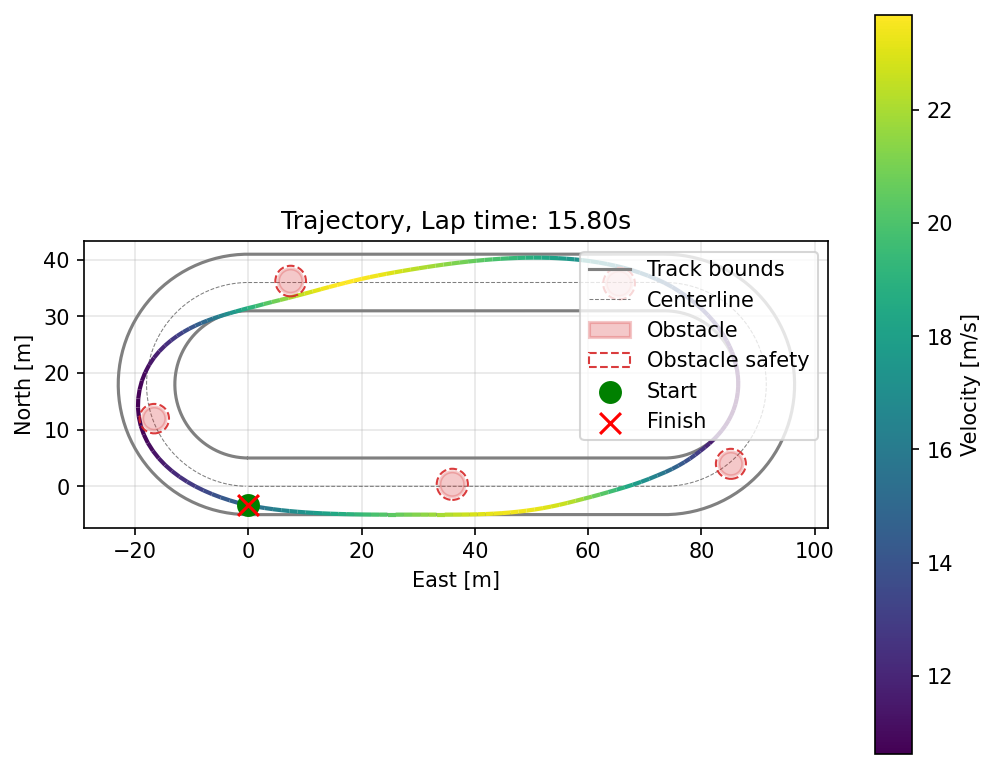
\includegraphics[width=\columnwidth]{img/ipopt_single_stage_trajectory.png}}
}{
\IfFileExists{fig_trajectory.png}{
\centerline{
\includegraphics[width=\columnwidth]{fig_trajectory.png}}
}{
\fbox{\parbox{0.95\columnwidth}{\vspace{0.4cm}\centering Trajectory figure not found.\vspace{0.4cm}}}
}
}
\caption{Representative IPOPT solution on the oval track with obstacles (current pipeline output).}
\label{fig:solver_output}
\end{center}
\vskip -0.2in
\end{figure}

%\textbf{Observed limitations.} Some adversarial obstacle placements still yield converged but unsafe trajectories (significant negative dense clearance) even after retries, indicating that (a) the current obstacle constraint discretization may be too coarse in extreme scenes, and (b) the initializer and/or constraint enforcement needs strengthening before large-scale dataset generation.

\section{Remaining work}
\label{sec:remaining}

\textbf{DT training and integration.}
(1) Train the Decision Transformer on RTG-conditioned sequences with track and obstacle features.
(2) Integrate DT outputs as IPOPT warm-start initializations $(X_0,U_0)$.

\textbf{Evaluation (final milestone).}
(3) Compare DT-warm-start vs.\ baseline initialization on: (i) IPOPT iterations, (ii) wall-clock solve time, (iii) acceptance rate without retries, and (iv) final lap time / constraint margins.

\bibliography{example_paper}
\bibliographystyle{icml2018}

\end{document}
